\section{Design}
\label{sec:research-one:design}

We present the design of \oursystem. We include Figure~\ref{fig:research-one:some-figure} and Table~\ref{tab:research-one:some-table}. We refer to subsections \S\ref{subsec:research-one:architecture} and \S\ref{subsec:research-one:optimizations}.


\subsection{Architecture}
\label{subsec:research-one:architecture}

Some text. Numbered enumeration in text: \circleb{1} option 1, \circleb{2} option 2, and \circleb{3} option 3. Some more text. Numbered enumeration in text with white background: \circlew{1} option 1, \circlew{2} option 2, and \circlew{3} option 3.

\paratitle{Some inlined title}
Some interesting dummy text. Some interesting dummy text. Some interesting dummy text. Some interesting dummy text. Some interesting dummy text. Some interesting dummy text. Some interesting dummy text. Some interesting dummy text. Some interesting dummy text. Some interesting dummy text.

Some interesting dummy text. Some interesting dummy text. Some interesting dummy text. Some interesting dummy text. Some interesting dummy text. Some interesting dummy text. Some interesting dummy text. Some interesting dummy text.

Some interesting dummy text. Some interesting dummy text. Some interesting dummy text. Some interesting dummy text. Some interesting dummy text. Some interesting dummy text. Some interesting dummy text.

\paratitlenodot{Some inlined title without dot} so the sentence continues with some interesting dummy text. Some interesting dummy text. Some interesting dummy text. Some interesting dummy text. Some interesting dummy text. Some interesting dummy text. Some interesting dummy text. Some interesting dummy text. Some interesting dummy text.

Some interesting dummy text. Some interesting dummy text. Some interesting dummy text. Some interesting dummy text. Some interesting dummy text. Some interesting dummy text. Some interesting dummy text. Some interesting dummy text.


\begin{figure}[t]
    \centering
    
    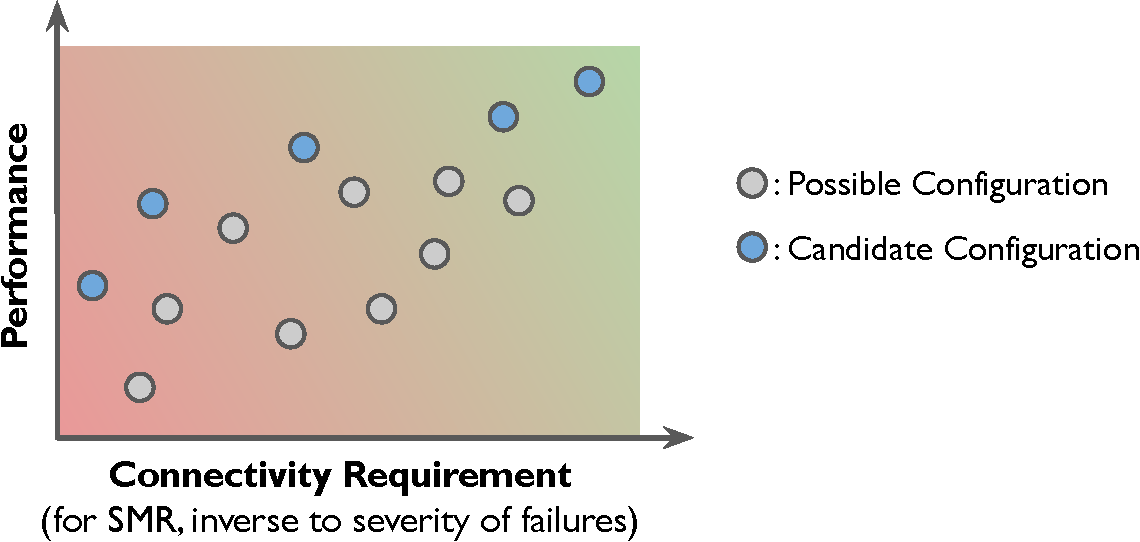
\includegraphics[width=0.75\textwidth]{images/research-one/example-plot.pdf}

    \floatcap{Some bold main figure caption}{Some auxiliary description in the caption.}
    
    \label{fig:research-one:some-figure}
\end{figure}



\subsection{Optimizations}
\label{subsec:research-one:optimizations}

Some text with a good-looking footnote\thesisfootnote{Here is a footnote.}.


\begin{table}[t]
    \centering
    
    \begin{tabular}{c|c|c}
        \hline \hline
            \textbf{System} &
            Features &
            Performance \\
        \hline \hline
            Ours &
            Many &
            Good \\
        \hline
            Existing &
            Few &
            Poor \\
        \hline \hline
    \end{tabular}

    \floatcapnodot{Some bold caption without trailing dot}{so the descriptive text continues in the same sentence which could be useful.}
    
    \label{tab:research-one:some-table}
\end{table}

